\documentclass[border=10pt]{standalone}
%%%<
\usepackage{verbatim}
%%%>
\begin{comment}
:Title: Polar plot of sine based function
:Tags: 2D;Functions;Polar Plots
:Author: Stefan Kottwitz
:Slug: sine-polar

The sine function is a well known periodic function. Choose an argument
factor, which doesn't divide the period well, and add another sine
function with a different factor, and you can see a complicated
path around the origin.

This plot was originally made for my blog post on TikZ.de:
http://tikz.de/periodisch/

See also the other polar sine plot examples there.
\end{comment}
\usepackage{pgfplots}
\usepgfplotslibrary{polar}
\begin{document}
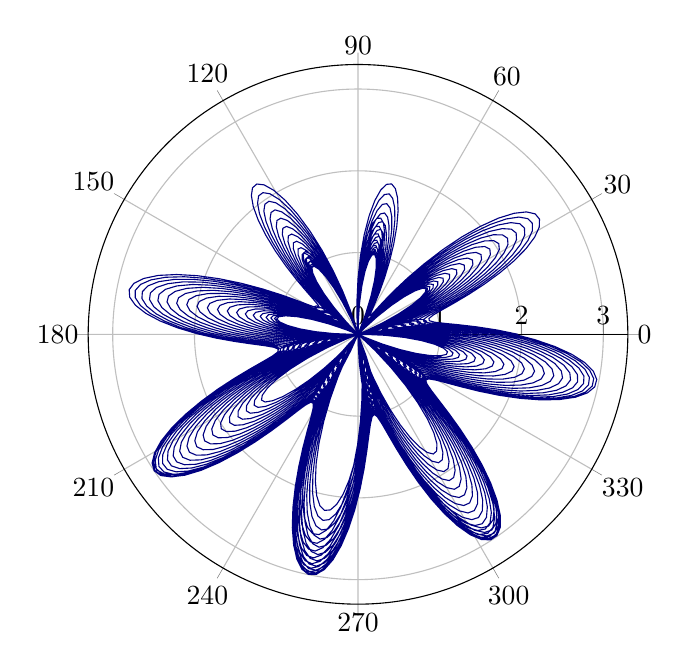
\begin{tikzpicture}
  \begin{polaraxis}[
      domain = -3600:3600,
      samples = 4000
    ]
    \addplot[blue!50!black] {1 - sin(50*x/49) - sin(8*x)};
  \end{polaraxis}
\end{tikzpicture}
\end{document}
